%%%%%%%%%%%%%%%%%%%%%%%%%%%%%%%%%%%%%%%%%
% Homework Assignment Article
% LaTeX Template
% Version 1.3.1 (ECL) (08/08/17)
%
% This template has been downloaded from:
% Overleaf
%
% Original author:
% Victor Zimmermann (zimmermann@cl.uni-heidelberg.de)
%
% License:
% CC BY-SA 4.0 (https://creativecommons.org/licenses/by-sa/4.0/)
%
%%%%%%%%%%%%%%%%%%%%%%%%%%%%%%%%%%%%%%%%%

%----------------------------------------------------------------------------------------

\documentclass[a4paper]{article} % Uses article class in A4 format

%----------------------------------------------------------------------------------------
%	FORMATTING
%----------------------------------------------------------------------------------------

\addtolength{\hoffset}{-2.25cm}
\addtolength{\textwidth}{4.5cm}
\addtolength{\voffset}{-3.25cm}
\addtolength{\textheight}{5cm}
\setlength{\parskip}{6pt}
\setlength{\parindent}{0in}

%----------------------------------------------------------------------------------------
%	PACKAGES AND OTHER DOCUMENT CONFIGURATIONS
%----------------------------------------------------------------------------------------

\usepackage{blindtext} % Package to generate dummy text
% \usepackage[style=numeric,sorting=none]{biblatex}
\usepackage{charter} % Use the Charter font
\usepackage[utf8]{inputenc} % Use UTF-8 encoding
\usepackage{microtype} % Slightly tweak font spacing for aesthetics

\usepackage[english]{babel} % Language hyphenation and typographical rules

\usepackage{amsthm, amsmath, amssymb} % Mathematical typesetting
\usepackage{float} % Improved interface for floating objects
\usepackage[final, colorlinks = true, 
            linkcolor = black, 
            citecolor = black]{hyperref} % For hyperlinks in the PDF
\usepackage{graphicx, multicol} % Enhanced support for graphics
\usepackage{xcolor} % Driver-independent color extensions
\usepackage{marvosym, wasysym} % More symbols
\usepackage{rotating} % Rotation tools
\usepackage{censor} % Facilities for controlling restricted text
\usepackage{listings, style/lstlisting} % Environment for non-formatted code, !uses style file!
\usepackage{pseudocode} % Environment for specifying algorithms in a natural way
\usepackage{style/avm} % Environment for f-structures, !uses style file!
\usepackage{booktabs} % Enhances quality of tables

\usepackage{tikz-qtree} % Easy tree drawing tool
\tikzset{every tree node/.style={align=center,anchor=north},
         level distance=2cm} % Configuration for q-trees
\usepackage{style/btree} % Configuration for b-trees and b+-trees, !uses style file!

% \usepackage[backend=biber,style=numeric,
            % sorting=nyt]{biblatex} % Complete reimplementation of bibliographic facilities
% \addbibresource{ecl.bib}
\usepackage{csquotes} % Context sensitive quotation facilities

\usepackage[yyyymmdd]{datetime} % Uses YEAR-MONTH-DAY format for dates
\renewcommand{\dateseparator}{-} % Sets dateseparator to '-'

\usepackage{fancyhdr} % Headers and footers
\pagestyle{fancy} % All pages have headers and footers
\fancyhead{}\renewcommand{\headrulewidth}{0pt} % Blank out the default header
\fancyfoot[L]{School of Computing, Macquarie University} % Custom footer text
\fancyfoot[C]{} % Custom footer text
\fancyfoot[R]{\thepage} % Custom footer text

\usepackage{comment}
\newcommand{\note}[1]{\marginpar{\scriptsize \textcolor{red}{#1}}} % Enables comments in red on margin

%----------------------------------------------------------------------------------------

\begin{document}

%----------------------------------------------------------------------------------------
%	TITLE SECTION
%----------------------------------------------------------------------------------------

\title{COMP3100 project report} % Article title
\fancyhead[C]{}
\hrule \medskip % Upper rule
\begin{minipage}{1\textwidth} % Center of title section
\centering 
\large % Title text size
Project report: Stage 2\\ % Assignment title and number
COMP3100 Distributed Systems, S2, 2022\\
\normalsize % Subtitle text size
SID: 4481 6936, Name: Jacob Temperley
%%%%\\ % Assignment subtitle
\end{minipage}
\medskip\hrule % Lower rule
\bigskip

%----------------------------------------------------------------------------------------
%	ARTICLE CONTENTS
%----------------------------------------------------------------------------------------
\section{Introduction}
This projects aim is to create a load balancing algorithm that meets a set of performance objectives that are derived from a set of predefined baseline algorithms. We will first define load-balancing, then outline the algorithms to compare against, and the performance metrics.\par
Load balancing is the process of assigning a series of jobs to a set of servers that con process them. Different algorithms can be used to assign the jobs to servers, and the characteristics of the jobs combined with the algorithm usually determines how effective different algorithms are, i.e. it is very rare that any single algorithm is ‘better’ than another in all cases.\par
We will be comparing the new algorithm to four existing algorithms: first-capable, first-fit, best-fit, and worst-fit. These algorithms are relatively simple, first-capable for example chooses the first server which is capable of running the current job regardless of whether it is already running a job. Understanding how these algorithms work can give us a starting point for building a new algorithm, and understanding what they don’t do can help us create better algorithms.\par
There are three performance metrics we can use to compare the effectiveness of our algorithms: average turnaround time, average resource utilisation, and total cost. Increasing the performance in one of these usually results in decreasing the performance in another, so will focus on decreasing the average turnaround time: the time between submission of a job, and the completion of that job.\par



\section{Problem definition}
\label{sec:section2}

If we have to sacrifice one performance metric to increase another, we have to make a decision on which we will focus on. We can rule out utilisation because of the way it is calculated; the baseline algorithms do not migrate jobs and servers are not simulating failures (at least I don’t think they are), which means the utilisation will always be 1, and we can’t have more than the maximum utilisation. That leaves turnaround time or cost.\par
Both average turnaround time and cost are valid focus’ when creating a new algorithm. Decreasing total cost would mean we have to know the individual cost of each server, then prioritise by cost. Unfortunately cost is only available through the xml configuration files that usually are specified when running ds-server, and without know the names of the files, becomes impossible. This leaves only turnaround time for our focus. \par



\section{Algorithm description}
How can we decrease the average turnaround time? Examining the baseline algorithms, it becomes clear that they all have one characteristic in common: they never migrate scheduled jobs to use resources that have been made available post-schedule. An example of this is depicted in figure 1, where we can see server 2 is unused for the majority of the simulation because the algorithm doesn’t identify that a resource has become available. Clearly job 3 could have been executed on server 2 in parallel with job 1 as in figure 2, but the order of scheduling prevents this. Having servers that sit idly by while jobs are waiting is a huge waste of time that increases the average waiting time. To achieve this effect with the simulator, we can listen for a JCPL message which notifies us a job has completed and a server might be idle. We can then use the MIGJ command to move a waiting job to an idle server.\par

\begin{figure}
    \centering
    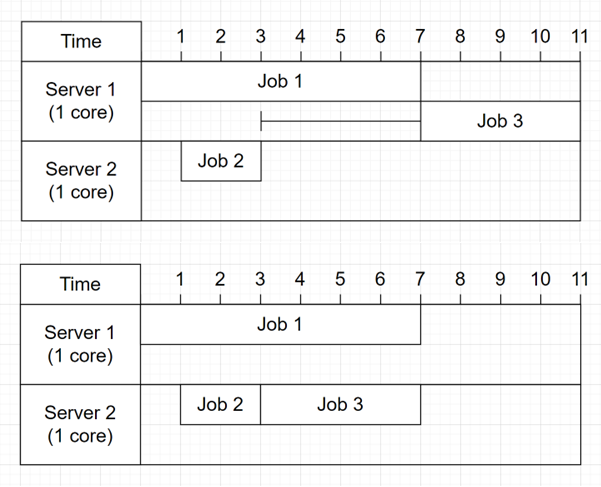
\includegraphics{migExample.png}
    \caption{An example of a scenario where migrating a waiting job (job 3) to an available server (server 2) decreases overall turnaround time.}
    \label{fig:example}
\end{figure}

What happens to the cost when we use a different server? Cost is calculated by multiplying the runtime by the server cost/second. If server 1 and 2 are of the same type, then regardless of where we place job 3 (behind job 1 or 2), the cost of running in either scenario does not change. Only when server 1 and 2 have different running cost will the total cost change. Using this principle, we can decrease the average turnaround time. \par

\section{Implementation}

The implementation for the check algorithm is relatively simple. The pseudo-code is as follows:\par

\begin{enumerate}
    \item Receive a job.
    \item Search for the first available server.
    \item If a server is available.
        \begin{enumerate}
            \item Assign a job to the server 
        \end{enumerate}
    \item Else
        \begin{enumerate}
            \item Assign the job to the first capable server.
        \end{enumerate}
    \item If a server becomes idle through completing a job
        \begin{enumerate}
            \item Find a waiting job that fits on the server.
            \item Migrate the waiting job to the idle server.
        \end{enumerate}
\end{enumerate}

\begin{figure}
    \centering
    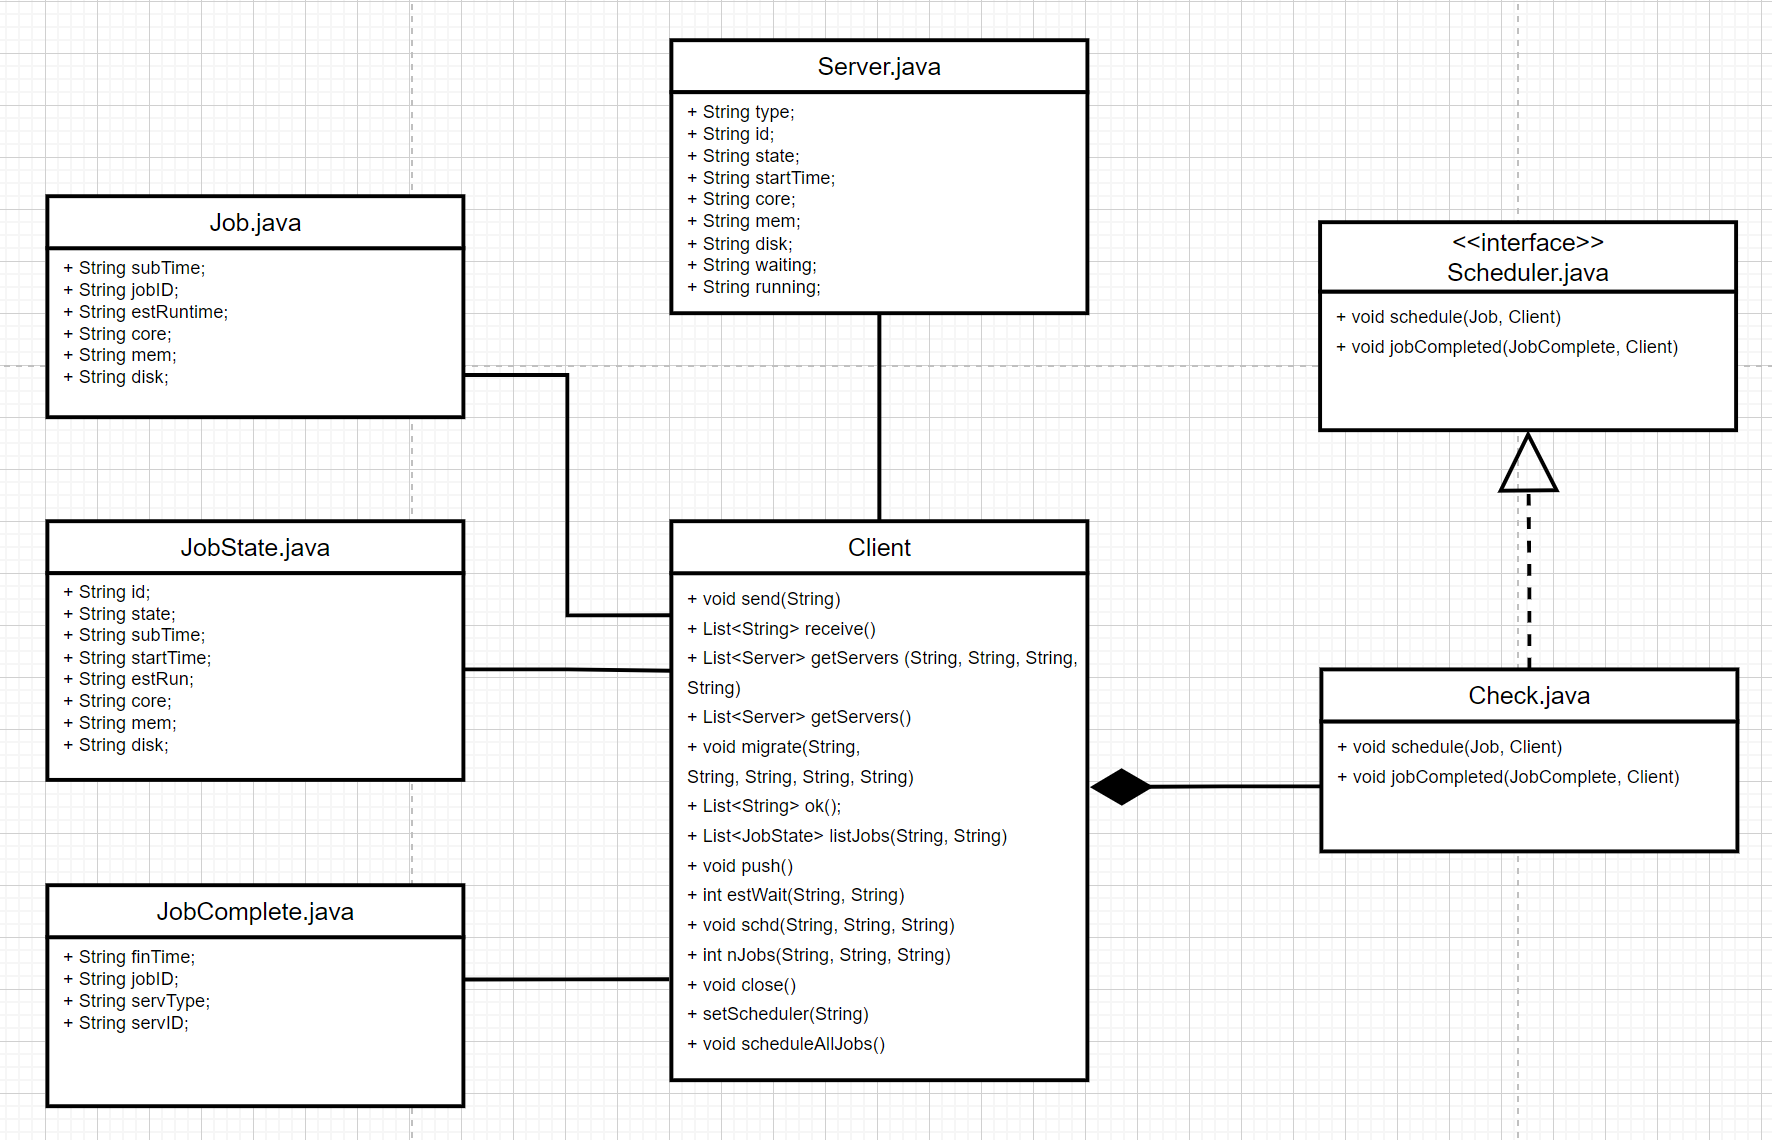
\includegraphics[scale=0.7]{class.png}
    \caption{The class diagram for the Client, Scheduler algorithm, and data structures used.}
    \label{fig:class}
\end{figure}


The class diagram for the algorithm implementation is in figure 3. The Client and Check classes are where the bulk of the functionality takes place; Client handles general ds-sim related messaging and program structure, Check contains the algorithm specific instructions like how to make scheduling decisions. The other classes are used as data structures to simplify ds-sim interaction, including Job, Server, JobState, and JobComplete. Generally, Client directly messages the simulation, receives messages in return, processes the information into data structures, and passes the data to a Scheduler.\par


\section{Results \& discussion}

The Check algorithm excels in turnaround time (figure \ref{fig:turn}), primarily through its use of job migration which allows jobs scheduling to adapt based on job completion. It can also adapt to realised running times, i.e. the algorithm can migrate jobs when the actual running time of a job is shorter or longer than the estimated runtime. Compared to the baseline algorithms which ‘fire-and-forget’, it seems obvious that considering the dynamic runtime environment will improve the turnaround time. \par

\begin{figure}
    \centering
    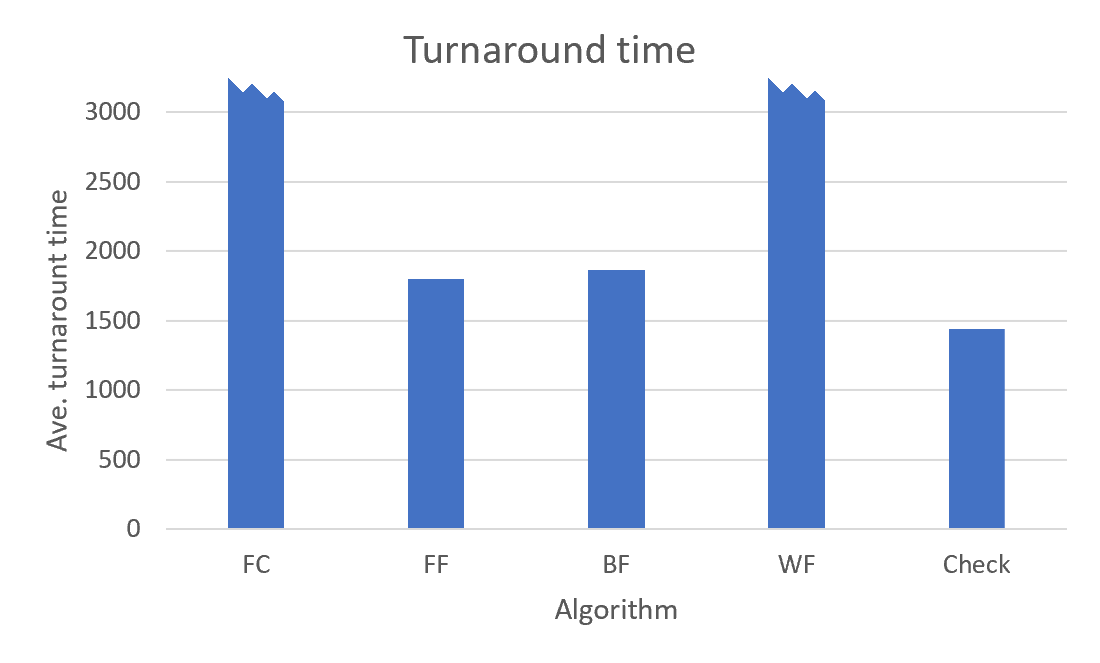
\includegraphics{turnGraph.png}
    \caption{The comparison of turnaround time (seconds) for baseline algorithms and the new Check algorithm.}
    \label{fig:turn}
\end{figure}

Comparing Check’s average utilisation (figure \label{fig:util}), we can see that its performance (63.71\%) is on-par with the baseline algorithms (FF = 63.3\%, BF = 60.72\%, WF = 68.79\%, FC = 94.37\%). This shows that our idea theory about negligent cost differences mostly works. There are hypothetical cases which increase the total cost; If a job completes on a 4-core server, searches for a waiting job, and finds a job which requires a single core, then 3 cores will be wasted where more jobs could have potentially run in parallel. Also, upgrading a job that would have run on a low cost server (but is currently unavailable) to a high cost (but available) server, will increase the cost of running the job and consequently the total cost.

\begin{figure}
    \centering
    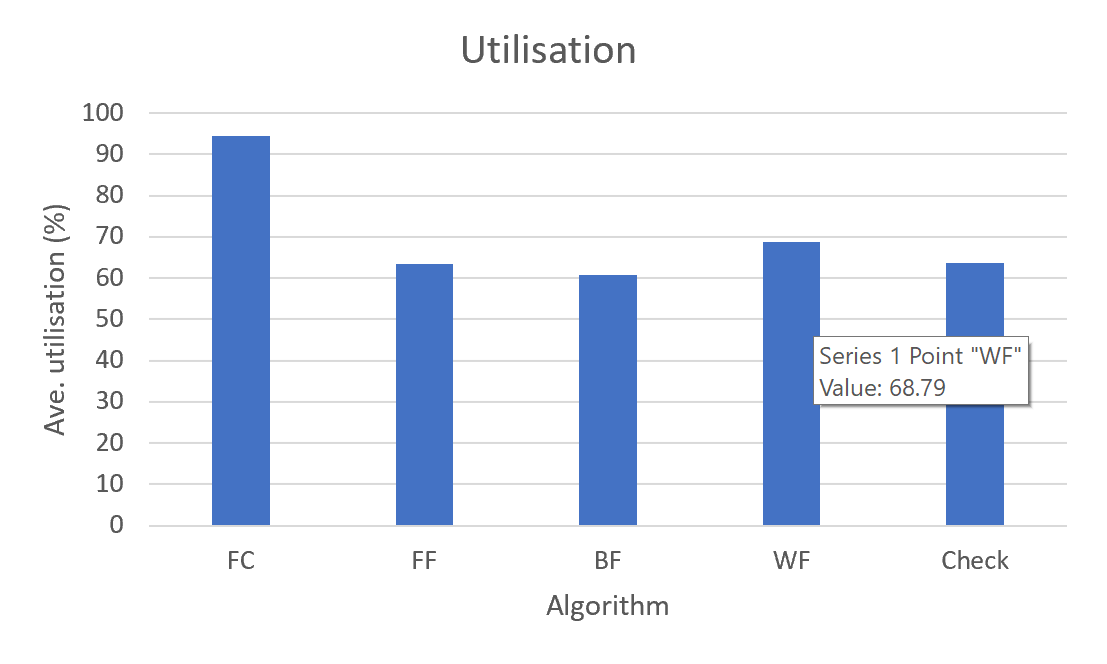
\includegraphics{utilGraph.png}
    \caption{The comparison of utilisation (percentage) for baseline algorithms and the new Check algorithm.}
    \label{fig:util}
\end{figure}

\begin{figure}
    \centering
    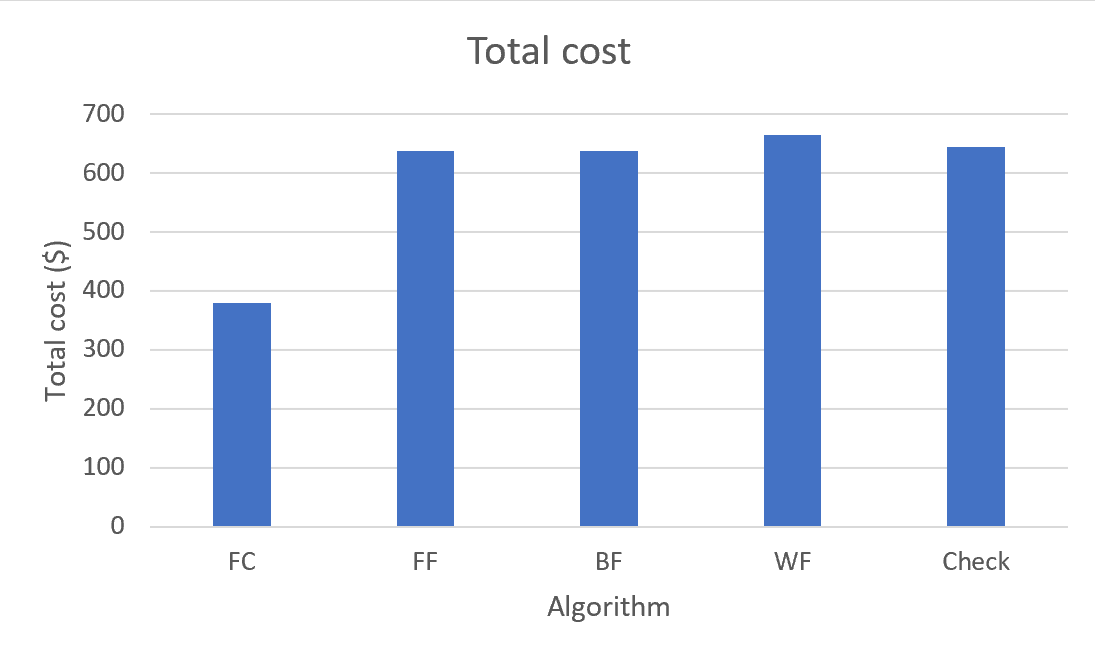
\includegraphics{costGraph.png}
    \caption{The comparison of total cost (\$) for baseline algorithms and the new Check algorithm.}
    \label{fig:util}
\end{figure}

Finally, cost is roughly on par with FF, BF, and WF, but all of these are almost double FC (figure \label{fig:cost}). If we consider that FC will only assign jobs to server types that have an ID of 0 (because IDs greater than 0 will never be the first discovered in a first capable search), then we can convince ourselves that a set of servers with multiples of each server type will only utilise a small fraction of the servers which minimises wasted server time. This goes hand-in-hand with high utilisation (FC = 94.37\%) which stands out from the rest of the baseline algorithms.\par
The cost resource wastage that potentially occurs could be countered by: finding multiple waiting jobs to run on large servers, using a best fit algorithm in tandem with Check to place the best job on completion, or both of the mentioned. If we do both, then we can place a best fitting job on an idle server and fill up leftover space with more concurrent jobs.




\section{Github link}
\url{https://github.com/jetemperley/COMP3100ass}
\end{document}
